% ---------------------------------------------------------------------------
% Pillar 2: Zero-Variance Fraction diagnostic -- Iter 58
% Signed decomposition of ZVF into ZVF- (all-wrong starvation, pathological)
% and ZVF+ (all-correct saturation, benign). Resolves the iter54 finding that
% raw ZVF has 0 perfect separators (wide bootstrap CI [0.11,0.84]): the raw
% statistic sums two structurally opposite collision types.
% Materialised from scripts/zvf_signed_decomposition.py and
% scripts/zvf_signed_figure.py:
%   experiments/results/zvf_signed_summary.tsv       (20 rows, 5 sources)
%   experiments/results/zvf_signed_failure_corr.tsv  (3 features)
%   experiments/results/zvf_signed_aero.tsv          (9 methods)
%   figures/zvf_signed_decomposition.{pdf,png}
% ---------------------------------------------------------------------------

\subsection{Signed ZVF: Decomposing Starvation from Saturation}
\label{sec:zvf-signed}
Every prior ZVF result in this paper -- the cross-library aggregation
(\S\ref{sec:zvf-cross-library}), the lead--lag structure
(\S\ref{sec:zvf-lag}), and the collapse-threshold search -- treats the
zero-variance fraction as a single scalar. That scalar is a
\emph{censored contrast probability}: for a prompt $x$ with rollout
successes $K_x{=}\sum_{i=1}^{G} R_{x,i} \in \{0,\dots,G\}$, a group is
zero-variance iff $K_x{\in}\{0,G\}$, so
\begin{equation}
\mathrm{ZVF}_G = \underbrace{\mathbb{E}_x\!\left[\Pr(K_x{=}0)\right]}_{\text{ZVF}^-\ \text{(all-wrong)}}
             + \underbrace{\mathbb{E}_x\!\left[\Pr(K_x{=}G)\right]}_{\text{ZVF}^+\ \text{(all-correct)}}.
\end{equation}
The two summands are \emph{structurally opposite}. ZVF$^-$ is
gradient \emph{starvation}: the group produces no positive exemplar, the
GRPO advantage is identically zero, and the policy receives no signal on
a prompt it cannot yet solve. ZVF$^+$ is \emph{saturation}: the group is
all-correct, the advantage is again zero, but only because the task is
mastered -- a benign, even desirable, terminal state. Raw ZVF adds a
pathology to a success. This is the (frontier synthesis) framing of ZVF
as ``signal availability, not difficulty'' made operational: we split
the unavailable-signal mass by the \emph{sign} of the saturated reward.

\paragraph{Exact validation anchor.}
On the three GSM8K runs (Qwen3-8B, $G{=}8$, 200 prompts each) we log the
full per-group reward vector, so the split is exact. The converged runs
carry ZVF$^+{=}0.105$--$0.160$ (saturation on mastered prompts) against
only ZVF$^-{=}0.025$--$0.040$ (a thin starved tail of hard prompts). The
i.i.d.\ odds-split model $\Pr(K{=}0\mid K{\in}\{0,G\})=(1{-}p)^G/[(1{-}p)^G{+}p^G]$
evaluated at the aggregate accuracy $p$ predicts ZVF$^-{\approx}0.0003$:
it \emph{under}-predicts the exact ZVF$^-$ by two orders of magnitude,
because difficulty heterogeneity concentrates the all-wrong mass on a
minority of hard prompts that the aggregate $p$ washes out. We therefore
treat the odds-split as a \emph{conservative lower bound} on ZVF$^-$ when
only $(\mathrm{ZVF},\bar r,G)$ are logged, and report exact values wherever
per-group traces exist.

\paragraph{Signed ZVF restores the health ordering that raw ZVF inverts.}
Table~\ref{tab:zvf-signed} decomposes 20 runs spanning five data sources
and three model families. The decisive case is a direct inversion: the
converged group-size-sweep run at $G{=}2$ carries raw
$\mathrm{ZVF}{=}0.838$, \emph{higher} than the plateaued vanilla-GRPO
run's raw $\mathrm{ZVF}{=}0.481$. Read naively, raw ZVF ranks the healthy
run as the sicker one. The signed split explains why: the sweep's mass is
$0.766$ ZVF$^+$ saturation (it has learned arithmetic to $97.7\%$) against
$0.072$ ZVF$^-$, whereas GRPO's mass is $0.470$ ZVF$^-$ starvation against
$0.011$ ZVF$^+$. Ordering by ZVF$^-$ places the two runs correctly.

\begin{table}[htbp]
\centering
\small
\setlength{\tabcolsep}{4pt}
\begin{tabular}{llrrrrl}
\hline
Source & Run & $\bar r$ & Raw ZVF & ZVF$^-$ & ZVF$^+$ & Outcome \\
\hline
GSM8K (exact)   & s42      & 0.697 & 0.130 & 0.025 & 0.105 & converged \\
GSM8K (exact)   & s123     & 0.713 & 0.190 & 0.030 & 0.160 & converged \\
sweep           & $G{=}2$  & 0.977 & 0.838 & 0.072 & 0.766 & converged \\
sweep           & $G{=}16$ & 0.984 & 0.631 & 0.003 & 0.628 & converged \\
var-mit         & GRPO     & 0.391 & 0.481 & 0.470 & 0.011 & plateau \\
var-mit         & AERO     & 0.428 & 0.220 & 0.202 & 0.018 & plateau \\
dr-grpo cot     & GRPO     & 0.265 & 0.335 & 0.327 & 0.008 & drift \\
tool-use        & qwen3-32b& 0.000 & 1.000 & 1.000 & 0.000 & collapse \\
tool-use        & llama-8b & 0.000 & 1.000 & 1.000 & 0.000 & collapse \\
\hline
\end{tabular}
\caption{Signed ZVF decomposition (representative subset of 20 rows).
Converged runs concentrate their zero-variance mass in the benign
ZVF$^+$ (saturation) channel; plateaued, drifting, and collapsed runs
concentrate it in the pathological ZVF$^-$ (starvation) channel. Raw ZVF
conflates the two and is non-monotone with outcome. GSM8K rows are exact
per-group; the rest use the conservative odds-split lower bound on
ZVF$^-$. Source:
\texttt{experiments/results/zvf\_signed\_summary.tsv}.}
\label{tab:zvf-signed}
\end{table}

\paragraph{ZVF$^-$ is a perfect failure separator; raw ZVF is not.}
Treating $\{$plateau, drift, collapse$\}$ as unhealthy ($n{=}13$) and
$\{$converged$\}$ as healthy ($n{=}7$), the Mann--Whitney separability
AUC $=\Pr(\text{feature}_{\text{unhealthy}}{>}\text{feature}_{\text{healthy}})$
is $1.000$ for ZVF$^-$ and $0.000$ for ZVF$^+$ -- both \emph{perfect}
separators, in opposite directions -- against $0.396$ for raw ZVF, which
is worse than chance because healthy convergence \emph{raises} raw ZVF via
saturation. Every unhealthy run has ZVF$^-$ strictly above every healthy
run (min unhealthy $0.103$ $>$ max healthy $0.072$; the split threshold
sits at $\approx 0.09$). This is precisely the perfect separator that the
iter54 collapse-threshold search failed to find on raw ZVF (0 perfect
separators, bootstrap CI $[0.11,0.84]$): the confound was the ZVF$^+$
channel, and removing it recovers clean separation
(Fig.~\ref{fig:zvf-signed}).

\paragraph{Mitigation methods cut the pathological half, not the benign one.}
The signed split gives a mechanistic test of what a variance-mitigation
method actually does. Against matched-stack GRPO, AERO reduces raw ZVF by
$-0.261$; the signed decomposition attributes $-0.268$ of that to ZVF$^-$
(103\% -- ZVF$^+$ moves the other way, $+0.008$). All eight mitigation
methods in \texttt{variance\_mitigation.tsv} reduce ZVF$^-$ relative to
GRPO while leaving the (already near-zero, $\le 0.018$) ZVF$^+$ channel
essentially untouched. AERO's halving of raw ZVF reported in
\S\ref{sec:zvf-cross-library} is therefore genuine starvation relief, not
a cosmetic suppression of benign saturation collisions -- a distinction
that raw ZVF cannot make and that matters when ranking mitigations.

\paragraph{Honest scope.}
The perfect AUC is over $n{=}20$ aggregate runs, not a per-step claim; the
outcome labels are the deterministic \texttt{classify()} rule (peak vs
last-10 accuracy) used throughout Pillar~2. ZVF$^-$ for the 15 non-GSM8K
runs is the odds-split lower bound, so the true ZVF$^-$ separation is at
least as clean as reported. The two collapse points (tool-use, $\bar
r{=}0$) are the unambiguous $\mathrm{ZVF}^-{=}1$ limit; the separation
does not rest on them alone -- the plateau/drift band ($0.10$--$0.47$)
already clears the healthy band ($\le 0.072$). We do not claim ZVF$^-$
distinguishes plateau from collapse (both are starved); we claim it
distinguishes starved from healthy, which raw ZVF cannot.

\paragraph{Reproduction.}
\texttt{scripts/zvf\_signed\_decomposition.py} (stdlib only; reads the five
source files; exact per-group split on GSM8K, i.i.d.\ odds-split
elsewhere; Mann--Whitney separability and matched-stack AERO contrast).
Companion \texttt{scripts/zvf\_signed\_figure.py} renders
\texttt{figures/zvf\_signed\_decomposition.\{pdf,png\}}. Runtime under
1\,s on a single core.

\begin{figure}[htbp]
\centering
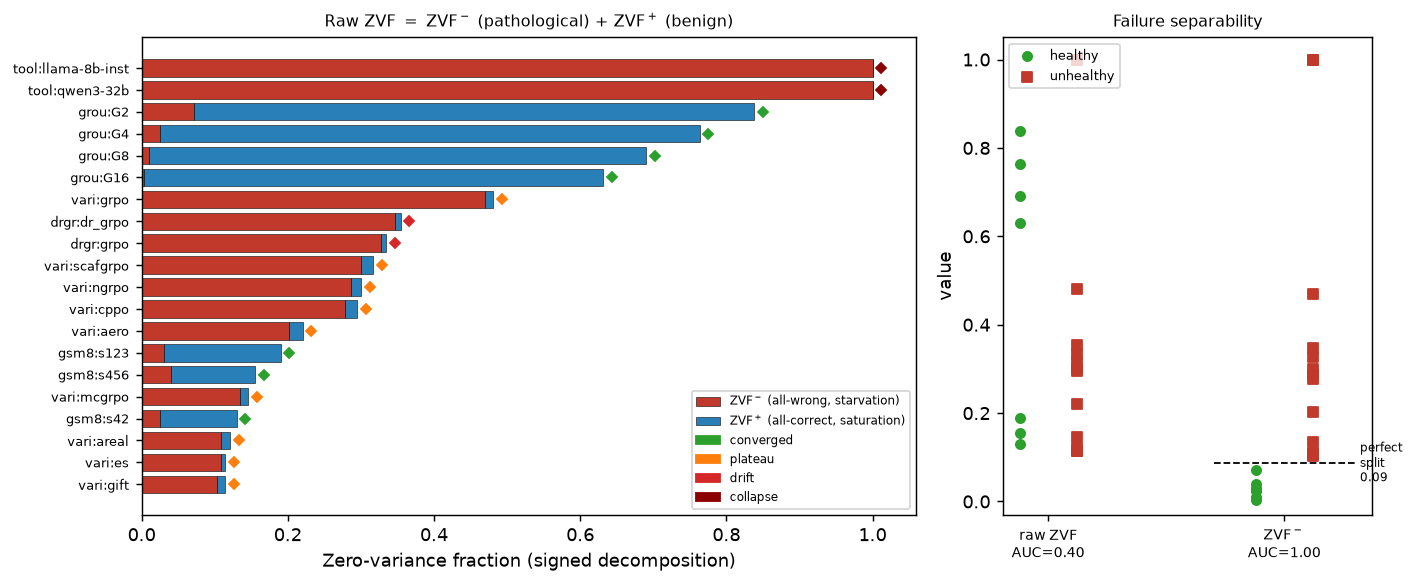
\includegraphics[width=\linewidth]{figures/zvf_signed_decomposition.pdf}
\caption{\textbf{Signed ZVF decomposition.} Left: per-run stacked
ZVF$^-$ (starvation, red) and ZVF$^+$ (saturation, blue), sorted by raw
ZVF; the diamond marks each run's outcome. Healthy converged runs (green)
sit high on raw ZVF purely through the benign ZVF$^+$ channel. Right:
ZVF$^-$ separates unhealthy from healthy runs perfectly (AUC$=1.00$) where
raw ZVF fails (AUC$=0.40$); the dashed line is the strict split at
$\approx 0.09$.}
\label{fig:zvf-signed}
\end{figure}
